\documentclass[final]{beamer}
%\usepackage{mathabx}
\usepackage{arev}

\usepackage{amsmath,amsthm,amssymb,latexsym,bbding}
\everymath{\displaystyle}
\usepackage{mathtools}
% \boldmath

\usepackage[utf8]{inputenc}
\usepackage{csquotes}
\usepackage[english]{babel}
\usepackage[T1]{fontenc}
\usepackage[orientation=portrait,size=custom, height=97,width=97,scale=0.93,debug]{beamerposter}
\mode<presentation>
  {
  \usetheme{IPFposter}
  }


%%%%%%%%%%%%%%%%%%%%%%%%%%%%%%%%%%%%%%%%%%%%%%%%%%%%%%%%%%%%%%%%%%%%%%%%%%%%%%
%% definitions for this poster only



%%%%%%%%%%%%%%%%%%%%%%%%%%%%%%%%%%%%%%%%%%%%%%%%%%%%%%%%%%%%%%%%%%%%%%%%%%%%%%
%% biblatex

\usepackage[backend=biber,citestyle=numeric-comp,bibstyle=BIBStyle,%
            sorting=none,doi=false,hyperref=false]{biblatex}
\bibliography{thebib}
\setbeamertemplate{bibliography item}[text]  % set bibliography item, to show 
                                             % the text of the item (as it 
                                             % comes from biblatex);
                                             % otherwise we get these little 
                                             % images



%%%%%%%%%%%%%%%%%%%%%%%%%%%%%%%%%%%%%%%%%%%%%%%%%%%%%%%%%%%%%%%%%%%%%%%%%%%%%%
%% length and layout stuff

\newlength{\columnheight}
\setlength{\columnheight}{97cm}

\setlength\textwidth{\paperwidth}

\newlength{\marginw}
\setlength{\marginw}{2cm}

\newlength{\tw}
\setlength{\tw}{\textwidth}
\addtolength{\tw}{-2\marginw}


\newlength{\colsep}
\setlength{\colsep}{2cm}

\newlength{\colw}
\setlength{\colw}{0.5\tw}
\addtolength{\colw}{-\colsep}


\setlength{\parindent}{0pt}

\setbeamersize{text margin left=0pt,%
text margin right=0pt,%
%sidebar width left=0pt,%
%sidebar width right=0pt,%
%description width=0pt,%
%description width of=0pt,%
%mini frame size=0pt,%
%mini frame offset=0pt%
}

\newenvironment{myTwoColPoster}{%
  \begin{minipage}[t]{\textwidth}%
    \hspace*{\marginw}%
    \hspace*{9.5bp}%  %% dirty trick!!!!
    %\hfill%
    \begin{minipage}[t]{\tw}}%
  {\end{minipage}%
   \hspace*{\marginw}%
   %\hfill%
   \end{minipage}}

\newenvironment{myCol}%
    {\begin{minipage}[t][\columnheight][t]{\colw}}%
    {\end{minipage}}

\newenvironment{textblock}[1]%
    {\begin{block}{\rule[-0.6ex]{0pt}{2.4ex}\raisebox{-0.25ex}[1.6ex]{#1}}%
     \vspace*{5mm}}%
    {\vspace*{5mm}\end{block}}


%%%------------------------------------------------------------------------%%%
%% the document
%%--------------------------------------------------------------------------%%

%% logos
\logoleft{\includegraphics[keepaspectratio=true,width=9cm]{fig/logos/dd1_1.pdf}}
\logoright{\includegraphics[keepaspectratio=true,width=9cm]{fig/logos/dd1_2.pdf}}

%% title
  \title[Fraktal Poster Sachsen]{{\huge Fraktale in Grenzen und Küstenlinien}}
  \author[]{\Large Dirk Romeis\inst{1} \and Ron Dockhorn\inst{1}
    \and Martin Wengenmayr\inst{1,2} \and Jens-Uwe Sommer\inst{1,2}} \institute[IPFdd UBS]{ \inst{1}Leibniz-Institut f\"ur
    Polymerforschung Dresden e. V., Hohe Stra\ss e
    6, 01069 Dresden\\
    \inst{2}TU Dresden, Intitut für Theoretische Physik, 01062 Dresden\\
    ~\vspace{1ex} } \date{}

%% set text in footline
\footlinetext{\texttt{http://www.ipfdd.de}\hfill\texttt{romeis@ipfdd.de, dockhorn@ipfdd.de, wengenmayr@ipfdd.de}}


%% replace altert{xx} command :
 %  "(\ \textcolor{IPFred}{.*?} )"  -->  " $1 "

%%--------------------------------------------------------------------------%%
%% content
\begin{document}
\begin{frame}[t]{}
\begin{myTwoColPoster}
% ---------------------------------------------------------%
% first column
\begin{myCol}
  \begin{textblock}{Wie lang ist die Grenze Sachsens?}
    \renewcommand{\baselinestretch}{1.4}
    \begin{minipage}[c]{0.99\textwidth}
      \begin{itemize}\setlength\itemsep{1.3em} \Large
        \item für Längenberechnung von \textit{ zackiger} Linie, wie K\"usten oder Grenzen ist die verwendete Aufl\"osung entscheidend
        \item \textcolor{IPFred}{Grenze} Sachsens: aus weiter Ferne durch ein \textcolor{IPFbrown}{Viereck} genähert \textbf{(Bild 1)}\\\vspace*{0.2cm}
        4 Punkte $\Rightarrow$ Grenze w\"are \textcolor{IPFred}{$591,4\,km$} lang
        \item Ranzoomen und Vermessung der Grenze mit:
        \begin{itemize}\large %\setlength\itemsep{1.1em}
          \item 8 Punkten $\Rightarrow$  \textcolor{IPFred}{$642,9\,km$} 
          \item 16 Punkten $\Rightarrow$  \textcolor{IPFred}{$718,2\,km$} 
          \item 32 Punkten  $\Rightarrow$  \textcolor{IPFred}{$780,1\,km$} \textbf{(Bild 2)}
          \item 64 Punkten $\Rightarrow$  \textcolor{IPFred}{$843,1\,km$} 
          \item 172 Punkten $\Rightarrow$  \textcolor{IPFred}{$945,5\,km$} 
          \item ca. 1150 Punkte $\Rightarrow$  \textcolor{IPFred}{$1251,8\,km$}  \textbf{(Bild 3)}
        \end{itemize}
      \end{itemize}
      \begin{center}
        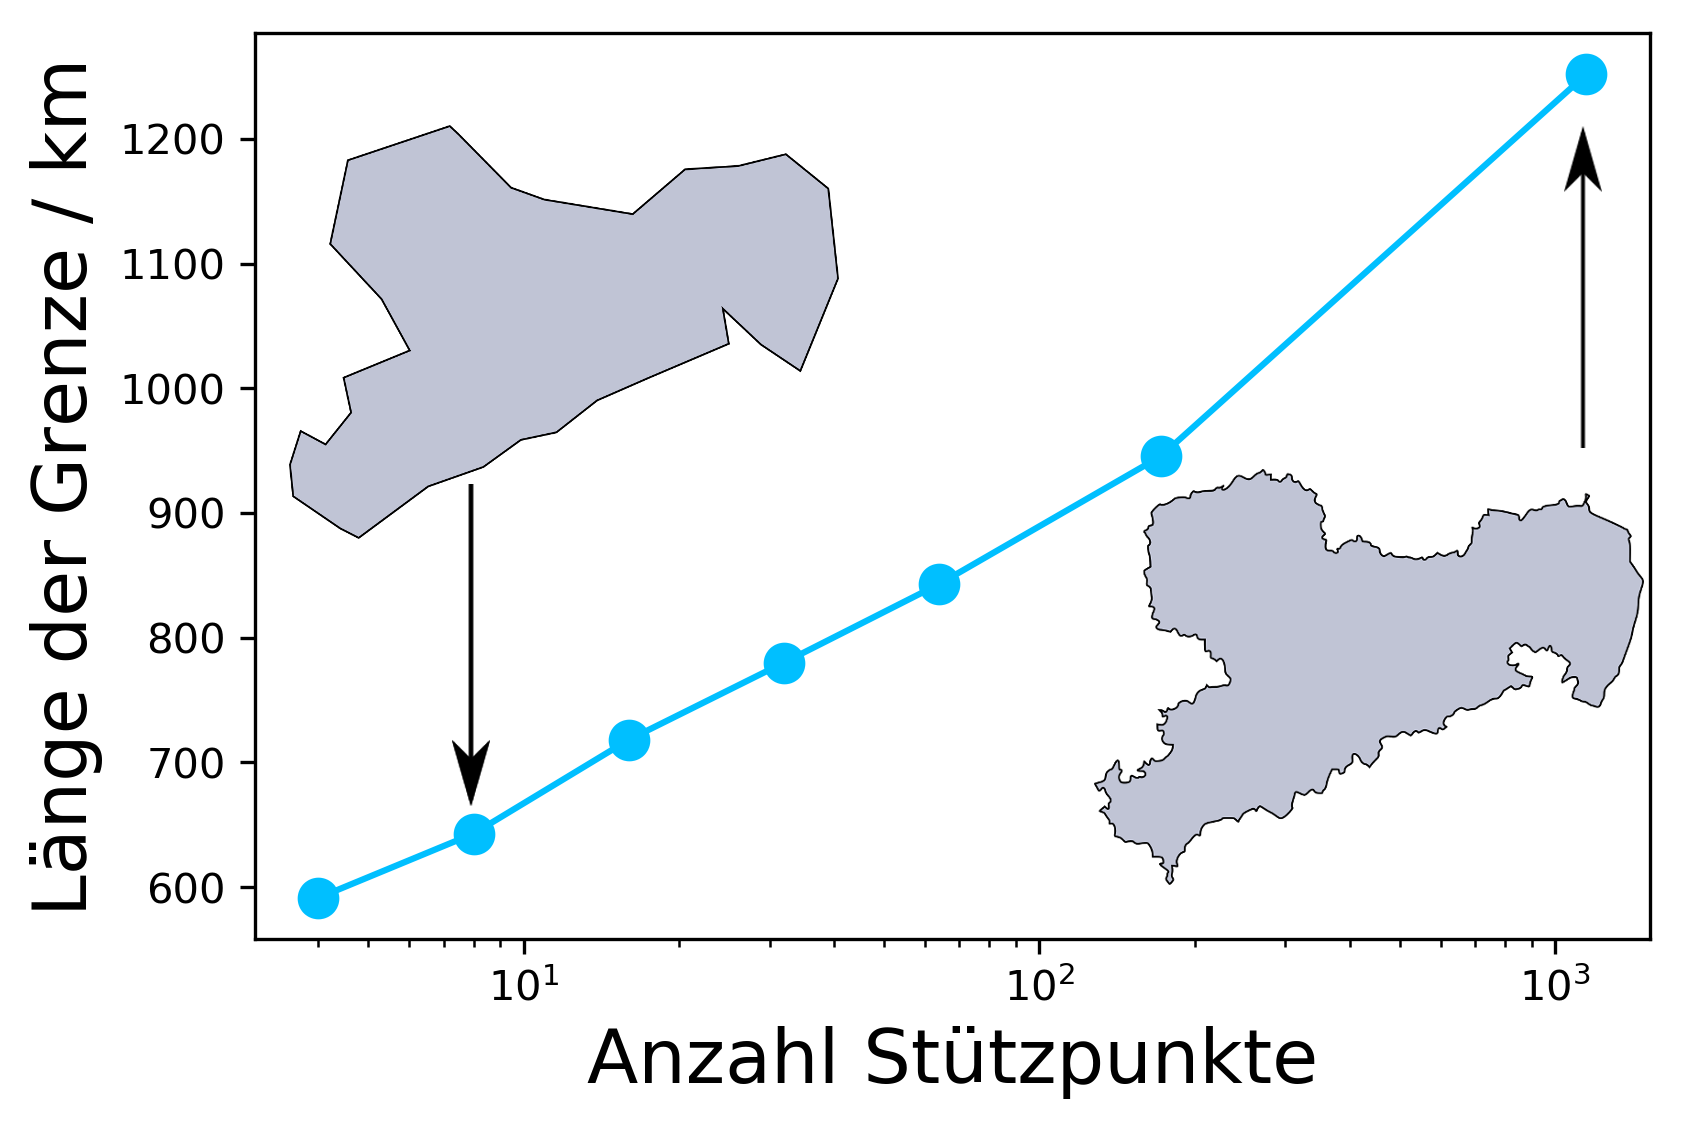
\includegraphics[width=0.75\textwidth]{fig/diag_punkte-laenge_insets}
      \end{center}
      \begin{itemize} \large \setlength\itemsep{1.2em}
        \item extrem detailierter Zoom \textbf{(Bild 4)} zeigt:
        \begin{center}
          \textbf{\textcolor{IPFbrown}{Die Grenze wird immer länger}}
        \end{center}
      \end{itemize}
      \begin{itemize} \large \setlength\itemsep{1.2em}
        \item \textbf{Eine scheinbar gerades St\"uck Grenze entpuppt sich bei genauerem Hinsehen als zackenf\"ormig und dessen Zacken haben selbst wieder Zacken ...}
        \item fraktale Eigenschaft: \textbf{\textcolor{IPFred}{Selbstähnlichkeit}}
        \item Wir berechnen f\"ur die Grenze Sachsens eine fraktale Dimension
      \end{itemize}
      \Large
      \begin{align*}
        \boldsymbol{D \approx 1,2 \neq 1}
      \end{align*}
    \end{minipage}

  \end{textblock}

  %%--------------------------------------------------------------------------%%
  \begin{textblock}{Konzept der Dimensionalit\"at}
    \large \textbf{  \textcolor{IPFred}{Intuitiv} } ist klar welche Dimension $D$ ein \textit{einfaches} geometrisches Objekt besitzt
    \begin{center}
        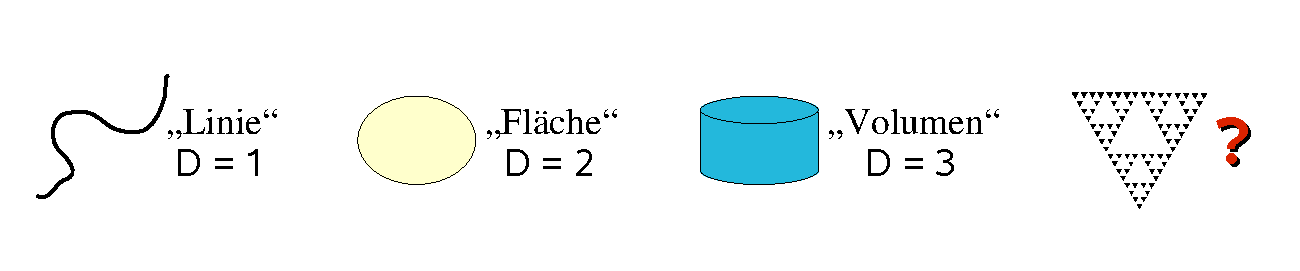
\includegraphics[width=0.8\textwidth]{fig/bsp}
    \end{center}
    \begin{center}
      \textit{L\"ange} einer Kugel oder \textit{Volumen} ein Rechtecks nicht sinnvoll definiert \\[1cm]
      {\Large \textcolor{IPFred}{ $\Rightarrow$ \textit{ Gr\"o\ss e} eines Objektes nur sinnvoll definiert im Bezug auf seine Dimension $D$}}
    \end{center}

  \end{textblock}
  %%--------------------------------------------------------------------------%%

  

\end{myCol}
% ---------------------------------------------------------%
% end the column
% \hspace*{\colsep}%
\hfill
% ---------------------------------------------------------%
% second column
\begin{myCol}
  
%%--------------------------------------------------------------------------%%

  %\end{textblock}
  %%--------------------------------------------------------------------------%%
  \begin{textblock}{Die Grenze in Bildern}

    \begin{minipage}[c]{0.75\textwidth}
      \begin{center}
        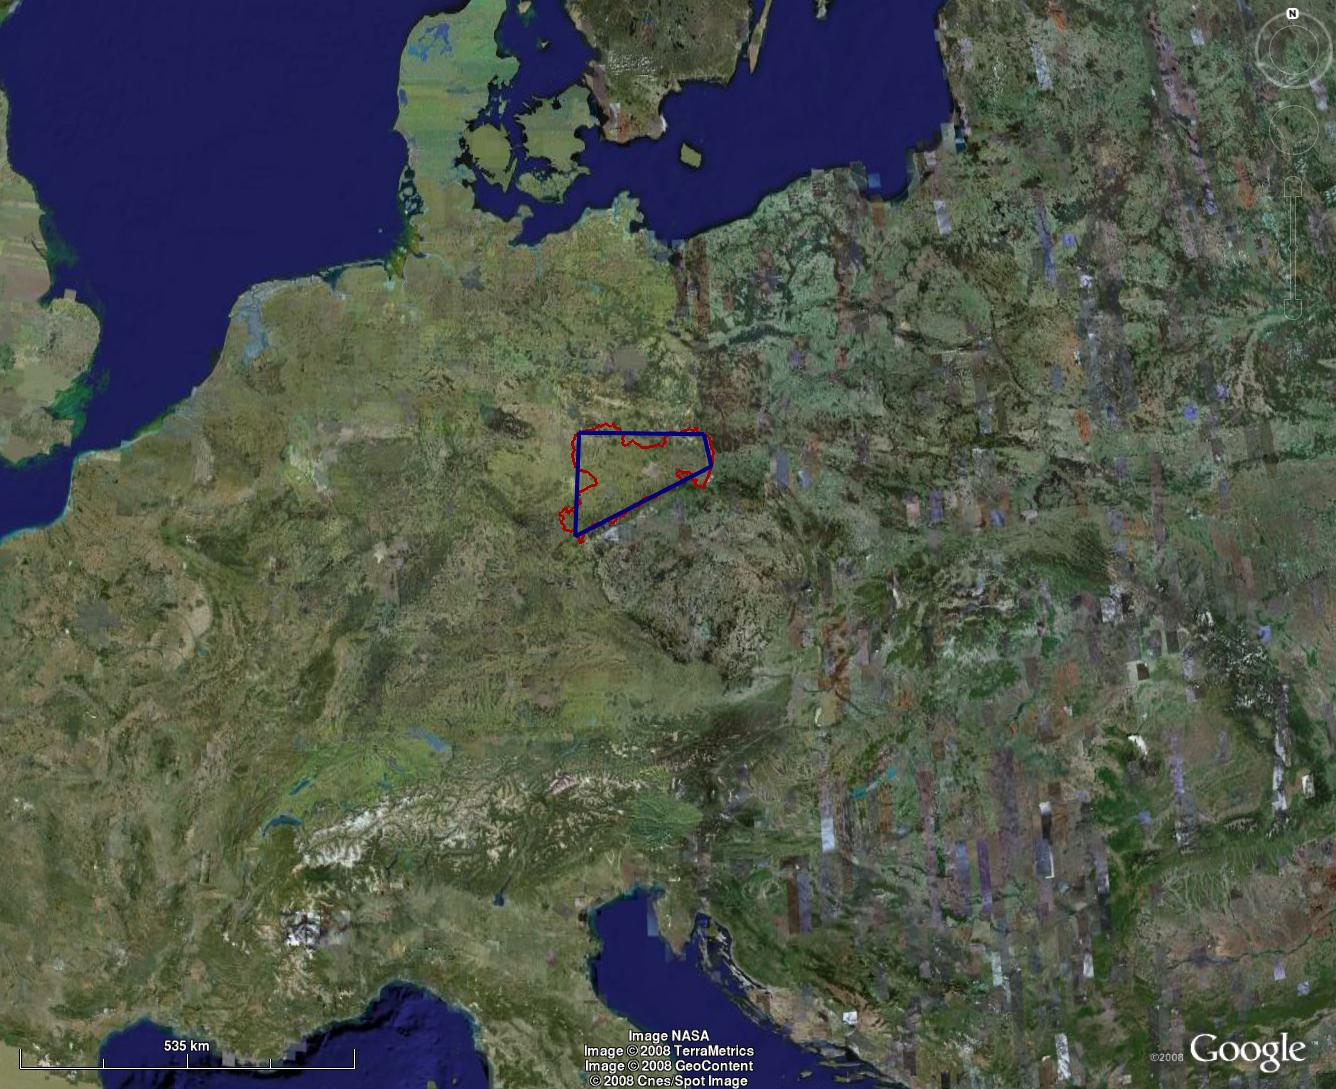
\includegraphics[width=0.71\textwidth]{maps/fern3}\\\vspace*{0.2cm}
        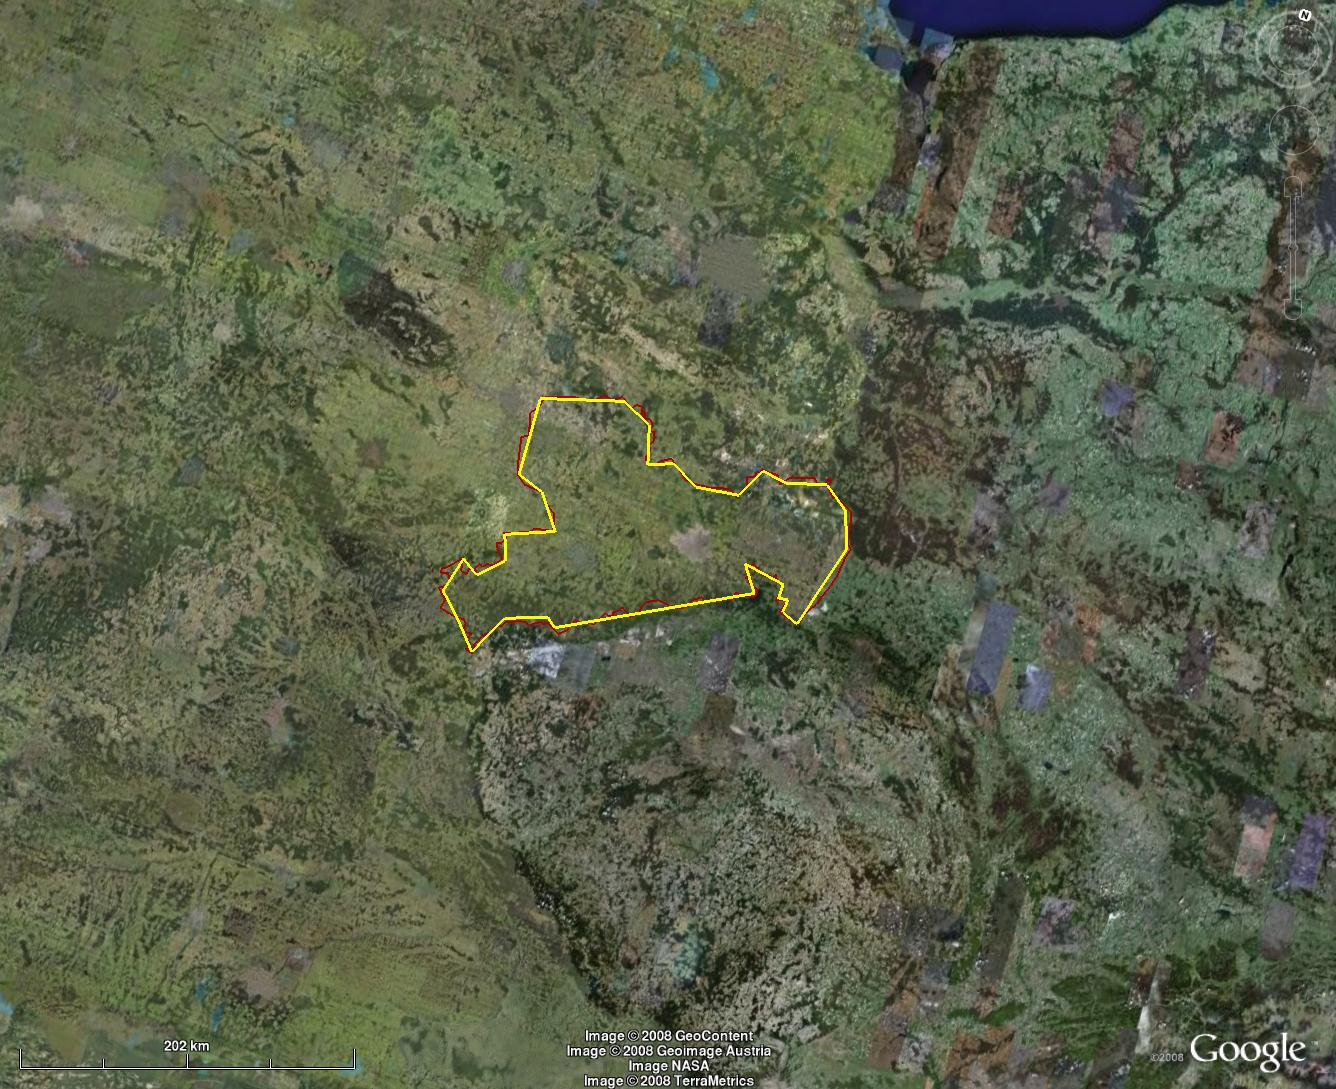
\includegraphics[width=0.71\textwidth]{maps/nahe}\\\vspace*{0.2cm}
        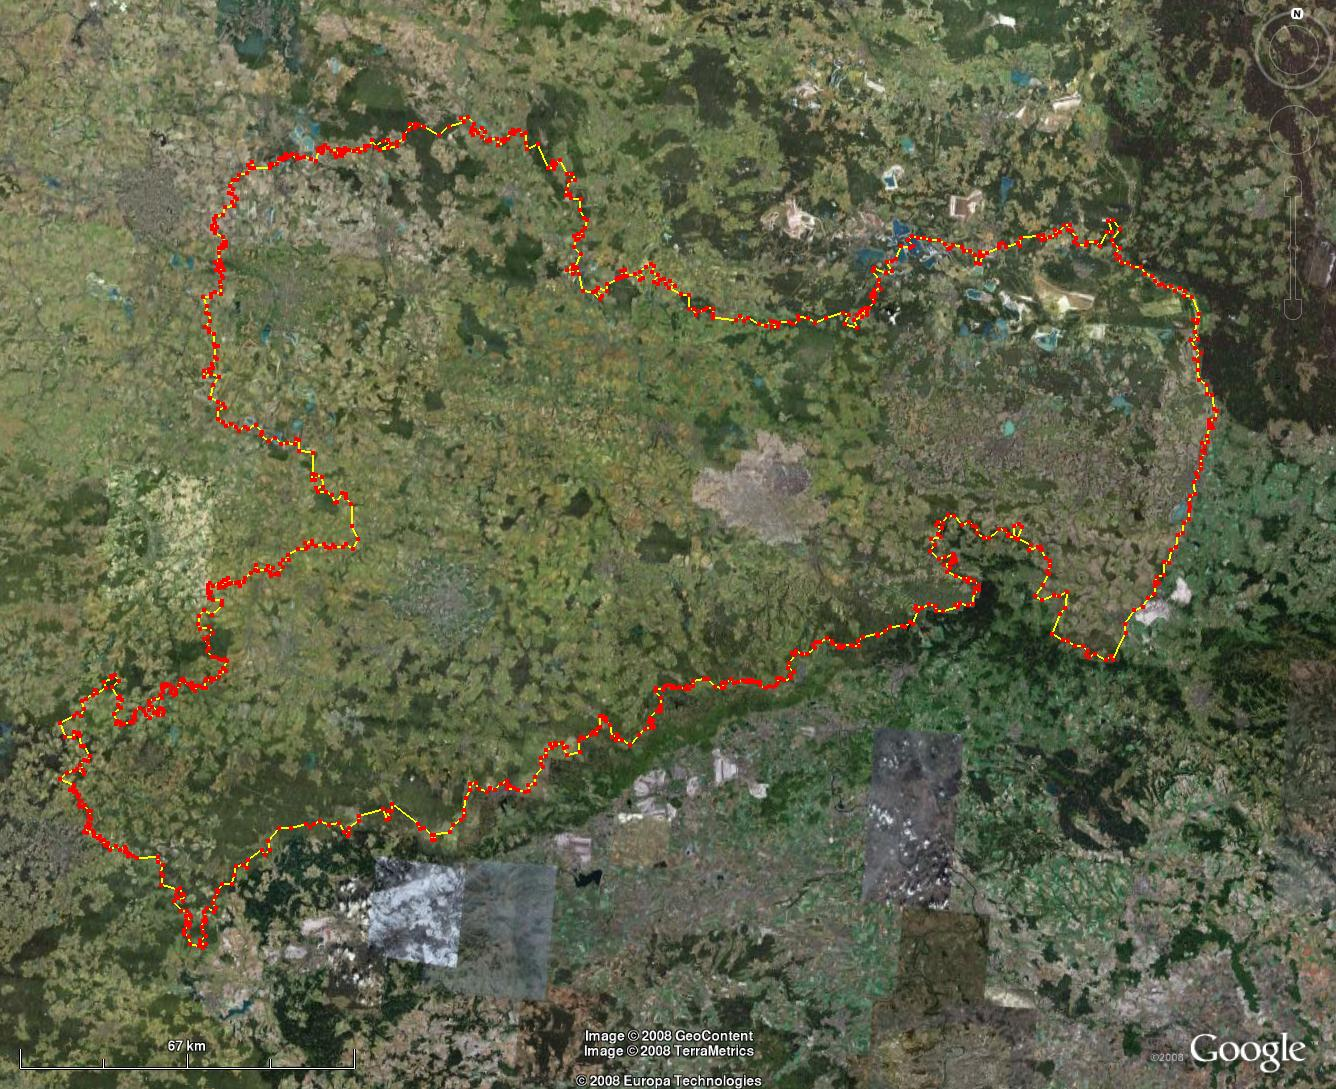
\includegraphics[width=0.71\textwidth]{maps/sa6}\\\vspace*{0.2cm}
        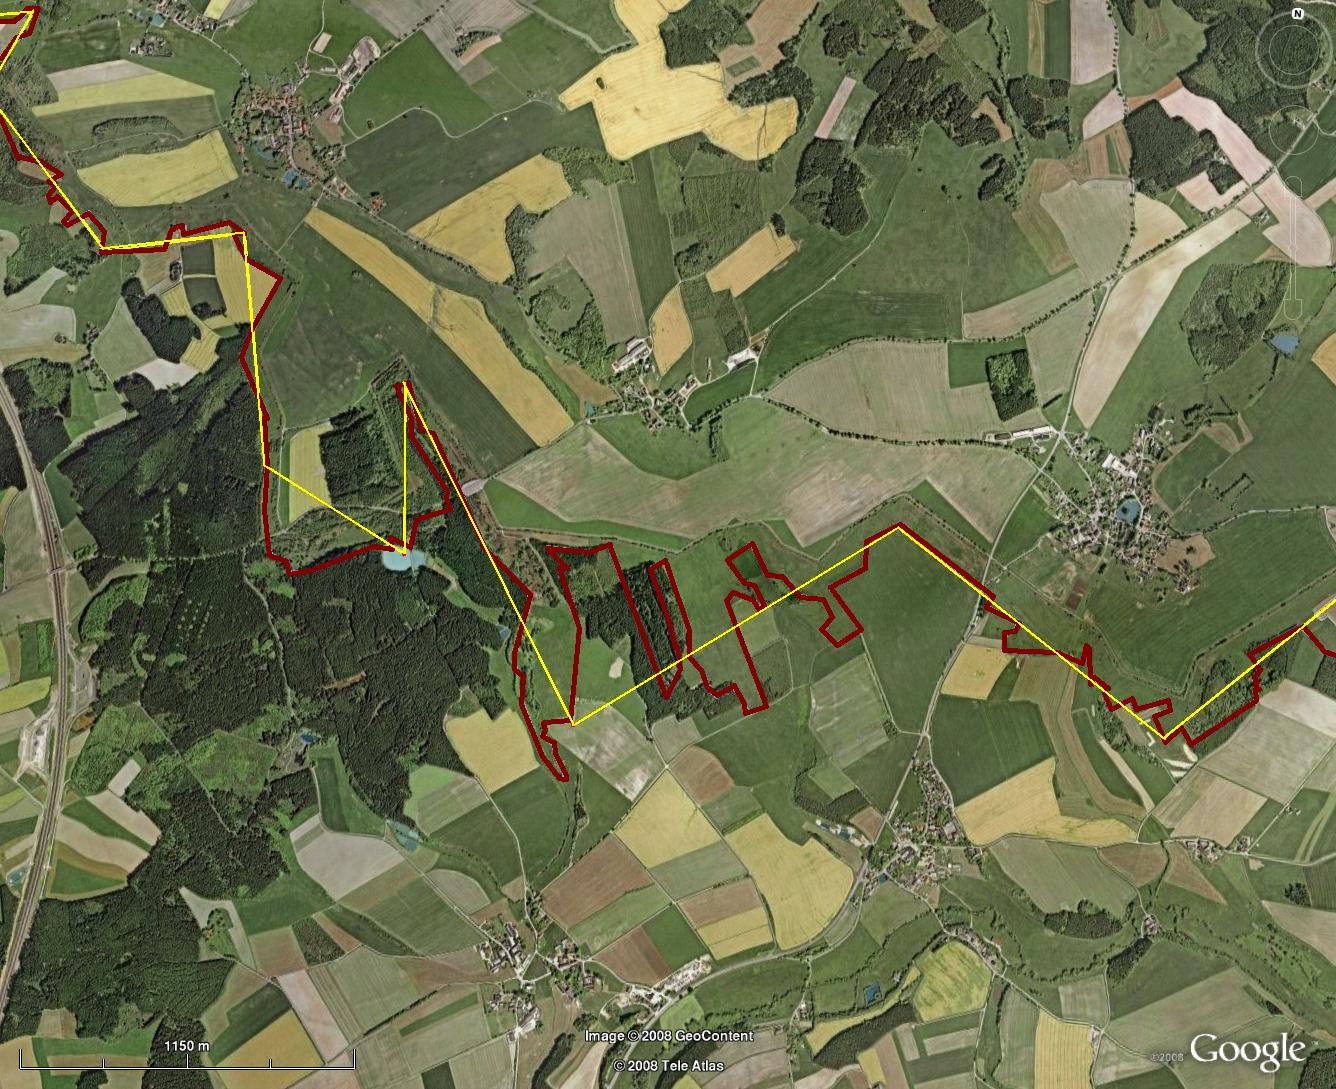
\includegraphics[width=0.71\textwidth]{maps/example}
      \end{center}
    \end{minipage}\hfill
    \begin{minipage}[c]{0.24\textwidth}
      \centering \Large
      \textbf{BILD 1 :}\\Sachsen aus der Ferne\\\vspace*{13.5cm}
      \textbf{BILD 2 :}\\Grenze mit 32 Punkten vermessen\\\vspace*{13.5cm}
      \textbf{BILD 3 :}\\Grenze mit ca. 1150 Punkten vermessen\\\vspace*{13.0cm}
      \textbf{BILD 4 :}\\Grenze regional\\{\normalsize(Grenzecke Sachsen-Bayern-Tschechien)}
    \end{minipage}


   \end{textblock}
   %%--------------------------------------------------------------------------%%


\end{myCol}%
\end{myTwoColPoster}
\end{frame}
\end{document}


%%% Local Variables:
%%% compile-command: "rake makepdf"
%%% End: